\section{Metadata}
\subsection{The Necessity for Formalized Persistence}

Having the results available from the Data Discovery tool, only during runtime is severely limiting.
Therefore, the output of the library must be persisted for later analysis.
Moreover, a standardized
metadata format is useful for data representation during runtime for other ad-hoc use cases.
\newline

A practical solution must adhere to several criteria.
Namely:
\begin{enumerate}
    \item It must use a pre-existing format.
    \item Low overhead.
    \item Minimal number of dependencies.
    \item Enforceable data-contract.
    \item Human readable.
\end{enumerate}

The requirement for the pre-existing format is an obvious one.
By using standardized formats such as XML we eliminate the need for custom tools to read the
data generated.

The second point is due to performance considerations. Generating and persisting the metadata must be
with as little disruption as possible, especially considering that IO resources may be limited as the
analysis is running.

The third condition is concerned with portability.
Ideally, the users of the library shouldn't be
forced to install any specialized applications just to read the metadata.
Enforcing this point also reduces the complexity of the Data Discovery tool

Having a data-contract allows the users to trust that the metadata follows certain constraints.
Therefore, the tools dependent on the data discovery library can rely on the metadata, and may generate their own,
to be fed back.

The last requirement, while not the most significant, enables the users to quickly understand the
state of the system, without having to rely on any helper tools.

\subsection{Representation Candidates}

Several options for metadata representation were considered, and each of them was evaluated by the above-detailed criteria.

\begin{enumerate}
    \item SQLite Database.
    \item Centralized metadata file(s).
    \item Individual metadata file for each analysed file.
\end{enumerate}

\textbf{Database approach:}
Initially, a local SQLite database was considered.
This option had many benefits, such as implicitly enforced data-contracts
in the form of the database schema.
Portability was also a benefit, as SQLite databases are encapsulated in a single file.

Performance would have been questionable, because on one hand DBMSes are optimized for multiple concurrent access,
but on the other hand, they inevitably introduce some overhead over simple file operations.

The main reason why this option was ultimately dropped, is that it would force the user to install software that
can access the generated databases.
Also, any other software that may want to consume the data generated will have to have an SQLite driver.

\textbf{Simple, file based approaches:}
Alternatively, the data discovery instance can simply write its results
to the disc, alongside the analysed data.
The output format will ideally follow some established standard such as XML
or JSON.

Of those two, the latter was picked due to its smaller overall footprint.
While XML has some great accompanying standards,
those are not particularly useful for simple data transfer.
The only necessary component is a way to validate the data.

Fortunately JSON schema is a well established option, and is suitable for the project's needs.

The only remaining decision left, was whether to have a centralized file, either on a project or on a folder level,
or to generate individual JSON files for each analysed file.

Having centralized files has the benefit of reduced footprint, and by extension -
better portability.

However, reading and writing into the same file throughout the discovery run is inefficient, and
needlessly complex, purely from a programmer's point of view.

This approach also fails from a readability standpoint, if we consider situations where the user
may only want to look at results from a particular file.

\subsection{Implementation}

Having decided on an approach, the next step was to introduce the metadata generation into the library.
Internally, the proper metadata structure is enforced by classes.

\begin{figure}[h]
    \centering
    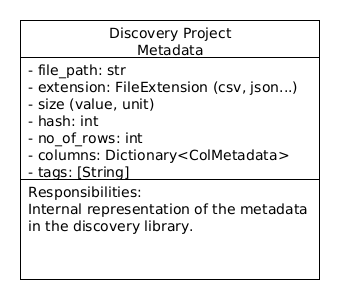
\includegraphics[width=6cm]{figures/metadata/metadata_class}
    \caption{Diagram for the class metadata}
    \label{fig:metadata_fig_1}
\end{figure}



\begin{figure}[h]
    \centering
    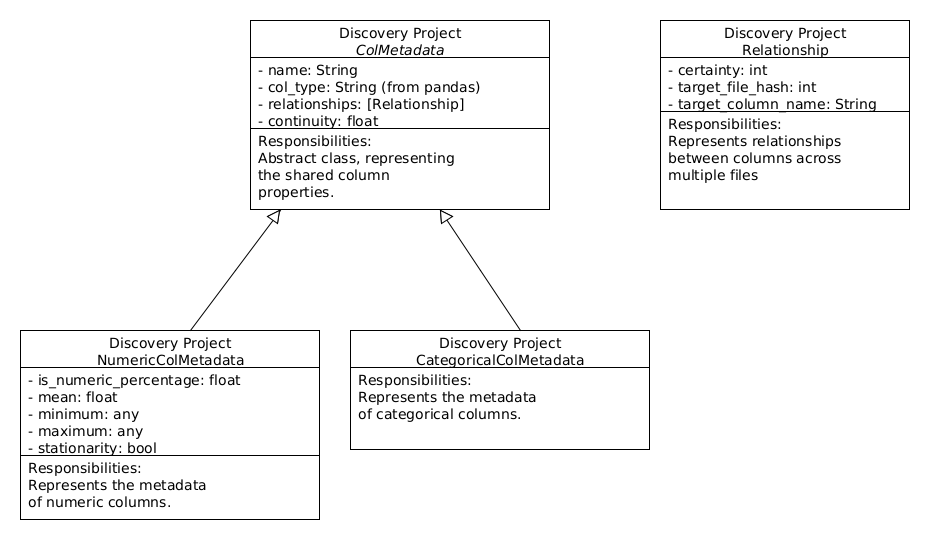
\includegraphics[width=12cm]{figures/metadata/col_rel_class}
    \caption{Diagram for the column and relationship classes}
    \label{fig:metadata_fig_2}
\end{figure}

The exact structure of these classes is as shown on figure ~\ref{fig:metadata_fig_1} and on figure ~\ref{fig:metadata_fig_2}.

After the analysis completes, the results are written into the same folder as the subject file.
The generated file's name has the format of \textit{name-of-the-subject-file.metadata.json}

\newline
\newline

An excerpt from a generated JSON file is as follows:
\begin{lstlisting}[language=json,firstnumber=1]
{
  "file_path": "/mock_filesystem/new_test_0.csv",
  "extension": "csv",
  "size": {
    "quantity": 1336720,
    "unit": "byte"
  },
  "hash": -7102791497049667481,
  "no_of_rows": 5000,
  "tags": [],
  "columns": [
    {
      "name": "Unnamed: 0",
      "is_numeric_percentage": 0.0,
      "continuity": 1.0,
      "mean": null,
      "minimum": "2016-01-01 00:00",
      "maximum": "2016-07-27 07:00",
      "stationarity": 0,
      "relationships": [
        {
          "certainty": 100,
          "target_file_hash": "1464446627197681099",
          "target_column_name": "Unnamed: 0"
        }
      ]
    },
\end{lstlisting}

A notable difference between the generated JSON files and the metadata classes is the
omission of the differentiation between categorical and numerical colum types.

This is due to a late realization, that often values that are not numerical may still have
\("\)numeric like\("\) values such as minimum and maximum. (e.g.\ dates), and those
were implicitly handled by the tools that implementation relies on.

\subsection{Data-Contract}
As detailed above, it is not enough to just make the metadata available for the users.
Its structure must adhere to a certain set of promises so that its consumers can reliably consume them.

The same principle must also be held up the other way around.
It's easy to reason that in the future third party plugins may be allowed to be part of
the library, in such situation, the library must ensure that the metadata it receives are valid.

Since it's already been established that the project will use JSON as its metadata format,
writing the data-contract in the form of a JSON schema standard ~\cite{jsonschema} was an obvious choice.

It's a simple format, also written in JSON. Moreover, due to its structure, it's human-readable, and self-explanatory.

Below is an excerpt from the JSON schema as implemented (full version is available in the appendix)
\begin{lstlisting}[language=json,firstnumber=1]
{
    "$schema": "http://json-schema.org/draft-04/schema#",
    "type": "object",
    "properties": {
    "file_path": {
      "type": "string"
    },
    "extension": { "enum": ["json", "csv", "parquet"] },
    "size": {
      "type": "object",
      "properties": {
        "quantity": {
          "type": "integer"
        },
        "unit": { "enum": ["byte", "kilobyte", "megabyte", "gigabyte"] }
      },
      "required": [
        "quantity",
        "unit"
      ]
\end{lstlisting}
\ldots
\begin{lstlisting}[language=json,firstnumber=1]
"relationships": {
  "type": "array",
  "items": [
    {
      "type": "object",
      "properties": {
        "certainty": {
          "type": "number",
          "min": 0,
          "max": 100
        },
        "target_file_hash": {
          "type": "string"
        },
        "target_column_name": {
          "type": "string"
        }
      },
      "required": [
        "certainty",
        "target_file_hash",
        "target_column_name"
      ]
    }
  ]
}
\end{lstlisting}

It's worth noting that this schema allows the use of custom JSON fields.
Therefore, it only enforces the inclusion of mandatory fields and the correct form of optional,
but handled fields.

Third party tools are able to add their custom data to the metadata files without making them invalid.
Naturally, in those cases the discovery library doesn't make any promises
about the proper handling of the custom fields.

In the concrete implementation, whenever a metadata file gets read, or written, the
subject string must, first pass through a validation layer before it's allowed to be consumed
or saved.

This behaviour also has the benefit of acting as an implicit test to ensure that library is working
as intended.